\documentclass[9pt,twocolumn,twoside]{pnas-new}
% Use the lineno option to display guide line numbers if required.

\usetikzlibrary{matrix, arrows.meta, positioning}

\articletype{SOCIAL SCIENCES / PSYCHOLOGICAL AND COGNITIVE SCIENCES}

\templatetype{pnasresearcharticle}

\begin{document}

\title{Role-Based Self-Organization as a Boundedly Rational Process}

\author[a,1]{Joseph Low}
\author[b]{Bhavyesh Sajja}
\author[b]{Tan Zhi-Xuan}

\affil[a]{Independent}
\affil[b]{National University of Singapore}

\leadauthor{Low}

\significancestatement{When humans cooperate---in a kitchen, a surgery, an
emergency response---they rarely coordinate by sharing a plan. Each person
infers what the others are doing and slots into a complementary role. We
introduce a controlled task in which three strangers must repeatedly divide
three roles among themselves under varying capability profiles, and develop a
Bayesian model that infers each teammate's role from their actions and
selects a role given those beliefs. Across 187 three-person teams, the best
account of human choices is a value-aware Bayesian model with a stickiness
bias: people reason about teammates and the expected value of each role, but
also resist switching. The result links ad-hoc role specialization to
Bayesian theory of mind.}

\authorcontributions{J.L. and T.Z.-X. designed the experimental platform.
B.S. and T.Z.-X. designed the computational model. J.L. and B.S.
analyzed the data. All authors contributed to the final manuscript.}
\authordeclaration{The authors declare no competing interests.}
\correspondingauthor{\textsuperscript{1}To whom correspondence should be addressed.
E-mail: jolow999\@gmail.com.}

\keywords{role specialization $|$ Bayesian theory of mind $|$ ad-hoc teamwork
$|$ cognitive modeling $|$ cooperation}

\begin{abstract}
Human teams cooperate effectively even when their members are strangers and
have never been told who does what. We propose that this capacity rests on
a Bayesian mechanism: each person maintains a probabilistic belief over
their teammates' roles, updates it from observed actions, and selects
their own role to maximize expected joint utility given those beliefs. We
test this account using a three-player online cooperative game in which
teams fight a series of bosses, choosing among three complementary roles
(Fighter, Tank, Medic) before each stage. Across 187 clean three-person
teams ($N{=}150$ participants), humans win 86\% of human rounds despite
stat-optimal play hovering near 50\% across stages---most teams find a
working role split that is not the stat-suggested one. A family of models
combining Bayesian inference about teammates' roles with utility-aware role
selection captures the team-level role distribution substantially better
than baselines (Pearson $r{=}0.50$ for the best model vs.\ $0.16$ for random
and $0.47$ for posterior-only). The best model adds an $\varepsilon$-mixture
stickiness term, consistent with humans being approximately Bayesian but
reluctant to switch roles. In bot ``deviation'' rounds, only 32\% of
participants reach the deviate-optimal role by the final stage despite
inferring their bot teammates' roles correctly. Ad-hoc role specialization
is well-described by a boundedly rational Bayesian theory of mind in which
the dominant departure from full rationality is behavioural stickiness
rather than poor inference.
\end{abstract}

\dates{This manuscript was compiled on \today}
\doi{\url{www.pnas.org/cgi/doi/10.1073/pnas.XXXXXXXXXX}}


\maketitle
\thispagestyle{firststyle}
\ifthenelse{\boolean{shortarticle}}{\ifthenelse{\boolean{singlecolumn}}{\abscontentformatted}{\abscontent}}{}

\Firstpage

\dropcap{H}umans routinely cooperate in groups whose members have never
worked together before. A surgical team that has not previously met still
divides itself smoothly between operator, anaesthetist, and scrub nurse;
strangers preparing a meal converge on chopper, stirrer, and washer within
minutes. This capacity for \emph{ad-hoc role specialization}---rapidly
inferring who is doing what and slotting into a complementary
role---underwrites much of human collective behaviour \cite{tomasello2014natural,
misyak2014unwritten}. Yet the cognitive mechanisms that support it remain
poorly understood. Two questions in particular are open: (i) how do people
infer their teammates' roles from limited behavioural evidence, and (ii)
how do those inferences feed into the choice of one's own role?

A growing body of work in computational cognitive science suggests that
social inferences are well-described as Bayesian reasoning over a
generative model of other agents
\cite{baker2017rational, ho2022planning, griffiths2010probabilistic}. This
approach has produced quantitatively accurate accounts of how people infer
others' beliefs and desires \cite{baker2017rational}, social norms
\cite{tan2019norms}, group membership \cite{davis2022inferring}, and
strategic types in repeated games \cite{lambaBayesianCoordination}. A
closely related literature on \emph{roles} as social categories has shown
that people use role labels to predict knowledge and behaviour rapidly and
efficiently \cite{bakerRolesGuideRapida, bakerPeopleUseMixed2025}, and that
roles in collaboration emerge in normatively predictable ways given task
structure \cite{mieczkowski2024specialization}. To our knowledge, however,
no existing study tests whether a Bayesian theory-of-mind model can
quantitatively predict the role choices of human teammates across a
controlled multiplayer task.

We address this gap with three contributions. First, we introduce an
\emph{experimental paradigm for ad-hoc role specialization}: a three-player
online cooperative game in which teammates choose between three
complementary roles (Fighter, Tank, Medic) at each stage of a multi-stage
boss fight, with stat profiles that asymmetrically favour different role \Endparasplit
combinations. Second, we develop a family of computational models that
treat role specialization as approximately rational action under
uncertainty: agents maintain a Bayesian posterior over teammates' roles,
update it from observed actions, and select roles by softmaxing over the
expected utility of the resulting team configuration. We benchmark this
model against posterior-only, value-only, threshold, and walk-style
alternatives, plus chance baselines. Third, we collected data from $N{=}150$
participants in three-person teams ($n{=}50$ games; 187 clean human team-rounds
and 258 bot-round trials), and compare model predictions against humans'
stage-by-stage role choices.

Our central finding is that a value-aware Bayesian model with a
stickiness bias---a ``Bayesian Walk''---best captures human role
choices at the team level (Pearson $r$ for joint role-combination
distribution = 0.50, vs.\ 0.47 for posterior-only and 0.16 for random),
and that the ranking is stable across three different evaluation metrics
(combination correlation, marginal correlation, and held-out
log-likelihood). The fitted stickiness term concentrates roughly half
the probability on the previously chosen role---consistent with the
empirically observed switch rate of 35--45\%. In bot-only rounds in
which the stat-suggested role differs from the team-optimal role, only
about a third of participants successfully deviated by the final stage,
despite reliably correct inferences about their bot teammates. Together
these results support a picture of ad-hoc role specialization as
\emph{boundedly rational Bayesian reasoning}: humans approximate optimal
inference and role selection, but their search through the space of role
assignments is biased by a strong preference for behavioural continuity.

\section*{An Ad-Hoc Role Specialization Task}\label{sec:task}

We introduce a three-player browser-based cooperative game implemented in
the Empirica framework \cite{empirica2021}. Teammates cannot
communicate, so coordination must proceed by inferring others' roles
from actions and choosing one's own role accordingly. We first describe
the task as a player encounters it, then give the formal MDP that
underlies it. The MDP supplies both the ground-truth labels used in
our behavioural analyses (\emph{stat-optimal} and
\emph{deviate-optimal} role assignments) and the value function that
will be plugged into the value-aware computational models below.
Neither of these is itself a cognitive hypothesis: they are properties
of the task.

\subsection*{Game as encountered by players.}\label{sec:task:structure}
Three players form a team that fights a single boss enemy across at
most five \emph{stages} per round (Fig.~\ref{fig:game}A). Each stage
unfolds in three phases. First, every player privately selects one of
three \textbf{roles}---\textit{Fighter}, \textit{Tank}, or
\textit{Medic}---which is revealed only through subsequent
actions. Second, two \textbf{turns} resolve in sequence; on each turn,
the chosen role determines the player's action through a deterministic
role policy (Fig.~\ref{fig:game}B): a Fighter always attacks; a Tank
blocks if the boss telegraphs an attack on this turn and otherwise
attacks; a Medic heals if the team has lost HP and otherwise attacks.
All three actions resolve simultaneously and update the team's and
boss's hit points (Fig.~\ref{fig:game}C). Third, an \textbf{inference
query} asks each player to guess which role each teammate was just
playing; these guesses are an explicit measurement of beliefs and do
not influence game dynamics. A round terminates when the team defeats
the boss (WIN), is reduced to zero HP (LOSE), or runs out of stages
(TIMEOUT, capped at five stages).

Each player is assigned a \textbf{stat profile}
$\theta_i = (\mathrm{STR}_i,\mathrm{DEF}_i,\mathrm{SUP}_i)$ that scales
the effectiveness of each role's signature action: STR scales Fighter
attacks, DEF scales Tank blocking, and SUP scales Medic healing.
Profiles are drawn from $\{(4,1,1),(1,4,1),(1,1,4),(2,2,2)\}$ and are
visible to all players throughout the round. Each profile therefore
suggests a \emph{stat-optimal} role---the role with the largest
signature stat---but players are free to deviate.

A game consists of six rounds split into two types
(Fig.~\ref{fig:game}D). In \textbf{human rounds} all three players are
real humans and the team must coordinate without communication. In
\textbf{bot rounds} the human plays alongside two AI bots whose roles
are fixed in advance to the team's \emph{deviate-optimal} assignment
(defined below), so the human must abandon their stat-suggested role to
fill the missing slot. Bot rounds isolate the question of whether
humans can override a strong prior cue when the joint optimum requires
it.

\begin{figure*}[t!]
\centering
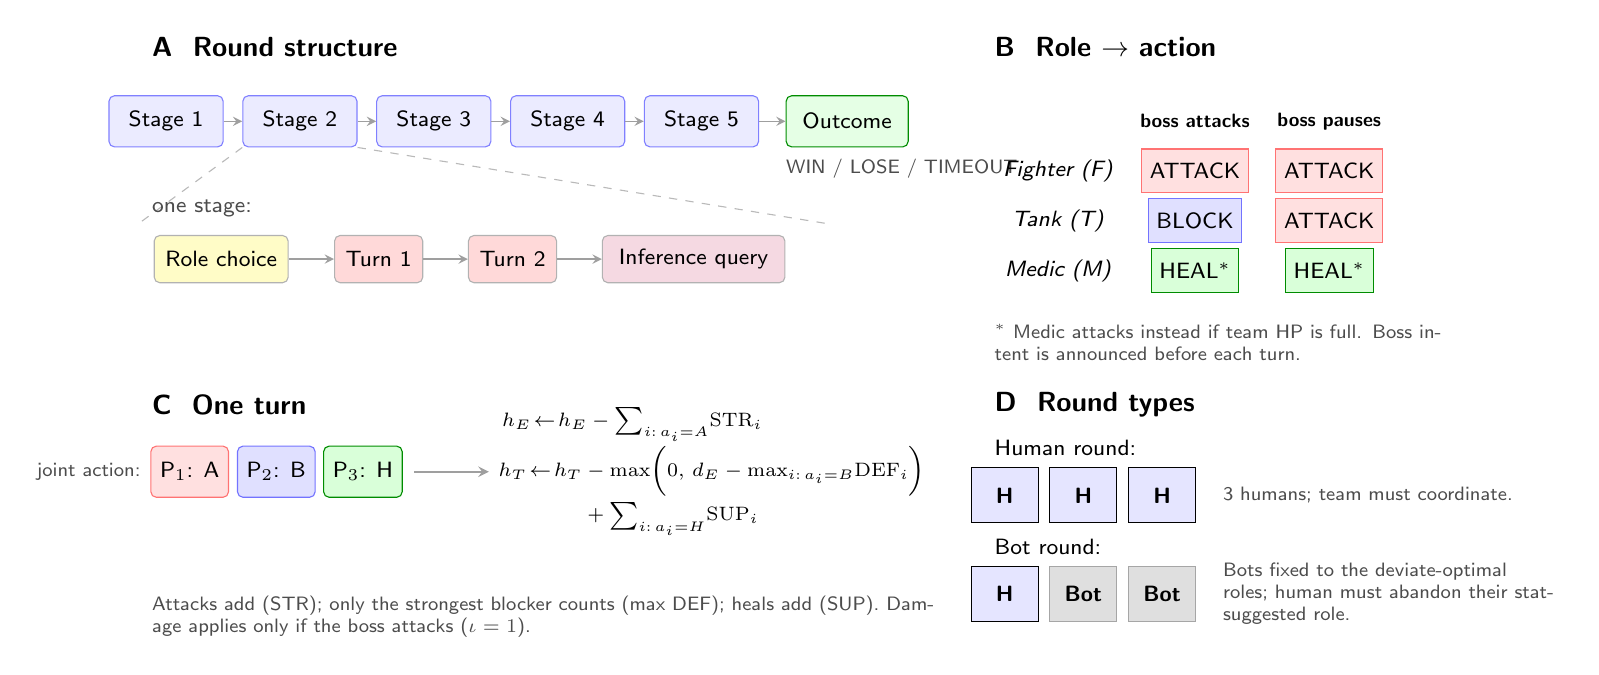
\begin{tikzpicture}[
  every node/.style={font=\sffamily\small},
  panel/.style={draw=gray!40, rounded corners=3pt, inner sep=8pt},
  ptitle/.style={font=\sffamily\bfseries},
  stage/.style={draw=blue!50, fill=blue!8, rounded corners=2pt,
                minimum width=1.45cm, minimum height=0.65cm,
                font=\sffamily\footnotesize},
  outc/.style={draw=green!55!black, fill=green!10, rounded corners=2pt,
               minimum width=1.55cm, minimum height=0.65cm,
               font=\sffamily\footnotesize},
  sub/.style={draw=gray!60, rounded corners=2pt,
              minimum height=0.6cm, font=\sffamily\footnotesize,
              inner xsep=4pt},
  arr/.style={->, >=stealth, gray!75, line width=0.5pt},
  fighter/.style={fill=red!12, draw=red!55},
  tank/.style={fill=blue!12, draw=blue!55},
  medic/.style={fill=green!15, draw=green!55!black},
  human/.style={draw=black, fill=blue!10,
                minimum width=0.85cm, minimum height=0.7cm,
                font=\sffamily\footnotesize\bfseries},
  bot/.style={draw=gray!70, fill=gray!25,
              minimum width=0.85cm, minimum height=0.7cm,
              font=\sffamily\footnotesize\bfseries},
]

% =================================================================
% Panel A: Round / stage / turn structure
% =================================================================
\node[ptitle, anchor=west] (Atitle) at (0,0) {\textbf{A}\ \ Round structure};

% Stage timeline
\foreach \i/\x in {1/0.3, 2/2.0, 3/3.7, 4/5.4, 5/7.1} {
  \node[stage] (S\i) at (\x,-0.95) {Stage \i};
}
\foreach \i/\nx in {1/2, 2/3, 3/4, 4/5} {
  \draw[arr] (S\i.east) -- (S\nx.west);
}
\node[outc] (out) at (8.95,-0.95) {Outcome};
\draw[arr] (S5.east) -- (out.west);
\node[anchor=west, font=\sffamily\scriptsize, gray!60!black]
     at (8.05,-1.55) {WIN / LOSE / TIMEOUT};

% Expanded stage detail (zoom-in)
\draw[dashed, gray!55] (S2.south west) -- (-0.05,-2.25);
\draw[dashed, gray!55] (S2.south east) -- (8.7,-2.25);
\node[anchor=west, font=\sffamily\footnotesize, gray!60!black]
     at (0, -2.05) {one stage:};

\node[sub, fill=yellow!22] (rc)  at (1.0,-2.7) {Role choice};
\node[sub, fill=red!15]    (t1)  at (3.0,-2.7) {Turn 1};
\node[sub, fill=red!15]    (t2)  at (4.7,-2.7) {Turn 2};
\node[sub, fill=purple!15, inner xsep=6pt] (inf) at (7.0,-2.7) {Inference query};
\draw[arr] (rc.east) -- (t1.west);
\draw[arr] (t1.east) -- (t2.west);
\draw[arr] (t2.east) -- (inf.west);

% =================================================================
% Panel B: Role policies
% =================================================================
\node[ptitle, anchor=west] at (10.7,0) {\textbf{B}\ \ Role $\to$ action};

\matrix (M) [matrix of nodes,
             anchor=north west,
             nodes={anchor=center, font=\sffamily\footnotesize,
                    minimum height=0.55cm, inner xsep=3pt},
             row sep=2pt, column sep=4pt,
             column 1/.style={nodes={font=\sffamily\footnotesize\itshape}},
             row 1/.style={nodes={font=\sffamily\scriptsize\bfseries}},
            ] at (10.7,-0.55)
{
                  & boss attacks & boss pauses \\
  Fighter (F)     & |[fighter]| ATTACK & |[fighter]| ATTACK \\
  Tank (T)        & |[tank]|    BLOCK  & |[fighter]| ATTACK \\
  Medic (M)       & |[medic]|   HEAL$^{*}$  & |[medic]| HEAL$^{*}$ \\
};
\node[anchor=north west, font=\sffamily\scriptsize, gray!60!black,
      text width=6cm]
     at (10.7,-3.4)
     {$^{*}$ Medic attacks instead if team HP is full. Boss intent is
      announced before each turn.};

% =================================================================
% Panel C: One turn's mechanics
% =================================================================
\node[ptitle, anchor=west] at (0,-4.55) {\textbf{C}\ \ One turn};

% Joint action panel
\node[draw=red!55,  fill=red!12,  rounded corners=2pt,
      minimum width=0.95cm, minimum height=0.65cm,
      font=\sffamily\footnotesize] (P1) at (0.6,-5.4) {P$_1$: A};
\node[draw=blue!55, fill=blue!12, rounded corners=2pt,
      minimum width=0.95cm, minimum height=0.65cm,
      font=\sffamily\footnotesize] (P2) at (1.7,-5.4) {P$_2$: B};
\node[draw=green!55!black, fill=green!15, rounded corners=2pt,
      minimum width=0.95cm, minimum height=0.65cm,
      font=\sffamily\footnotesize] (P3) at (2.8,-5.4) {P$_3$: H};

\node[anchor=east, font=\sffamily\scriptsize, gray!60!black]
     at (P1.west) {joint action:};

% Arrow
\draw[arr, line width=0.7pt] (3.45,-5.4) -- (4.4,-5.4);

% Mechanics
\node[anchor=west, font=\sffamily\scriptsize, text width=5.6cm]
     at (4.4,-5.4)
     {\,$h_E \!\leftarrow\! h_E - \sum_{i:\,a_i=A}\!\mathrm{STR}_i$ \\[1pt]
      $h_T \!\leftarrow\! h_T - \max\!\big(0,\, d_E - \max_{i:\,a_i=B}\!\mathrm{DEF}_i\big)$ \\[1pt]
      $\hphantom{h_T \!\leftarrow\! h_T} + \sum_{i:\,a_i=H}\!\mathrm{SUP}_i$\,};

\node[anchor=north west, font=\sffamily\scriptsize, gray!60!black, text width=10cm]
     at (0,-6.85)
     {Attacks add (STR); only the strongest blocker counts (max DEF); heals add (SUP).
      Damage applies only if the boss attacks ($\iota=1$).};

% =================================================================
% Panel D: Round types
% =================================================================
\node[ptitle, anchor=west] at (10.7,-4.55) {\textbf{D}\ \ Round types};

% Human round
\node[anchor=west, font=\sffamily\footnotesize] at (10.7,-5.1) {Human round:};
\node[human] (H1) at (10.95,-5.7) {H};
\node[human] (H2) at (11.95,-5.7) {H};
\node[human] (H3) at (12.95,-5.7) {H};
\node[anchor=west, font=\sffamily\scriptsize, gray!60!black,
      text width=4.3cm]
     at (13.6,-5.7) {3 humans; team must coordinate.};

% Bot round
\node[anchor=west, font=\sffamily\footnotesize] at (10.7,-6.35) {Bot round:};
\node[human] (HB) at (10.95,-6.95) {H};
\node[bot]   (B1) at (11.95,-6.95) {Bot};
\node[bot]   (B2) at (12.95,-6.95) {Bot};
\node[anchor=west, font=\sffamily\scriptsize, gray!60!black,
      text width=4.3cm]
     at (13.6,-6.95)
     {Bots fixed to the deviate-optimal roles; human must
      abandon their stat-suggested role.};

\end{tikzpicture}
\caption{Overview of the ad-hoc role specialization task. (\textbf{A})
A round consists of up to five stages, each comprising a private role
choice, two turns of joint action, and an inference query in which the
player guesses each teammate's current role. (\textbf{B}) Roles map
deterministically to actions through a role-conditioned policy that
depends on the announced boss intent and current team HP.
(\textbf{C}) On each turn the three players' actions resolve
simultaneously: attacks (A) are additive in STR, blocks (B) are
sub-additive in DEF (only the strongest blocker counts), and heals
(H) are additive in SUP. (\textbf{D}) Human rounds feature three
humans; bot rounds replace two of them with bots whose roles are
fixed to the deviate-optimal assignment, so the human must override
their own stat-suggested role.}
\label{fig:game}
\end{figure*}

\subsection*{The task as a Markov Decision Process.}\label{sec:task:mdp}
A single round is a finite-horizon MDP parametrised by the team's stat
profile $\theta_{1:3}$, the boss's pre-committed attack-intent sequence,
and a horizon $H$ (turns to the end of the round).

\paragraph*{State and action.} The state $s = (\iota, h_T, h_E)$ holds
the boss's announced intent for the upcoming turn
($\iota \in \{0,1\}$, common knowledge), the team's HP $h_T$, and the
boss's HP $h_E$. A state is terminal if $h_T=0$ or $h_E=0$. The joint
action is $a = (a_1,a_2,a_3) \in \{\mathrm{ATTACK},\mathrm{BLOCK},\mathrm{HEAL}\}^3$;
the three components resolve simultaneously into the HP updates shown
in Fig.~\ref{fig:game}C.

\paragraph*{Role-conditioned action model.} Each role induces a
deterministic preferred action $a^*(r,s)$: Fighter $\to$ ATTACK; Tank
$\to$ BLOCK iff $\iota=1$, else ATTACK; Medic $\to$ HEAL iff
$h_T < h_T^{\max}$, else ATTACK. We assume action noise:
\begin{equation}\label{eq:action-noise}
P_\varepsilon(a \mid r, s) =
\begin{cases} 1-\varepsilon & a = a^*(r,s),\\
\varepsilon/2 & \text{otherwise.}\end{cases}
\end{equation}

\paragraph*{Reward and team value function.} A round yields reward
$R = 100\,(t/H)$ when the team ends a stage with $h_T > 0$ and
$h_E = 0$ (a fast win is rewarded more than a slow one); otherwise
$R=0$. For any joint role assignment $\mathbf{r} = (r_1,r_2,r_3)$ and
state $s$, the team's expected return under the role-conditioned policy
is
\begin{equation}\label{eq:value}
V(\mathbf{r}, s) \;=\;
\mathbb{E}\!\left[\sum_{t=0}^{H} R(s_t) \;\middle|\; s_0=s,\;
a_t \!\sim\! \textstyle\prod_i P_\varepsilon(\cdot \mid r_i, s_t)\right].
\end{equation}
We pre-compute $V$ by exact value iteration on the tabular MDP,
separately for each $(\theta_{1:3}, \text{intent sequence})$
configuration used in the experiment (Methods).

\paragraph*{Stat-optimal vs.\ deviate-optimal.} The \emph{stat-optimal}
role assignment matches each player to the role their stat profile
favours; the \emph{deviate-optimal} assignment is
$\arg\max_{\mathbf{r}} V(\mathbf{r}, s_0)$. In most stat profiles these
coincide, but a subset (used in bot rounds) was chosen so that the two
disagree---the stat-suggested role is sub-optimal for the team.
$V(\mathbf{r},s)$ is a property of the task; it tells us the expected
payoff of any role assignment if every player follows the
role-conditioned policy. It is not a model of cognition. We will use
$V$ in two roles below: (i) as the ground truth that defines
deviate-optimal assignments, and (ii) as a fixed input to those
cognitive models that hypothesise humans are value-aware.

\section*{Computational Models}\label{sec:models}

We model each player as an approximately Bayesian agent that maintains
a posterior over teammates' role assignments, updates it from the
observed action history, and uses it to choose their own role at the
next stage. Within this family we vary two design choices---whether
role selection consults the task's value function $V$, and whether the
agent is sticky in its own role---yielding seven models
(Table~\ref{tab:models}). All seven share the same inference module
(below) and differ only in the role-selection rule.

\subsection*{Belief over teammates' roles.}\label{sec:models:inference}

\paragraph*{Prior.} Before observing any actions, the agent has a
structured prior driven by the (common-knowledge) stat profiles:
\begin{equation}\label{eq:prior}
P_0(r_1,r_2,r_3 \mid \theta_{1:3}) \propto \exp\!\left(\frac{1}{\tau_p}
\sum_{i=1}^3 \theta_i[r_i]\right),
\end{equation}
where $\theta_i[r_i]$ is the stat in $\theta_i$ corresponding to role
$r_i$ (e.g.\ STR for Fighter) and $\tau_p$ controls how strongly the
prior follows the stats. This captures the intuition that, before
observing any actions, teammates are more likely to be playing roles
their stats favour.

\paragraph*{Likelihood and posterior update.} The likelihood reuses the
MDP's role-conditioned action model
(Eq.~\ref{eq:action-noise}). After each turn, the joint posterior over
the role triple is updated by Bayes' rule using the observed joint
action and the current game state.

\paragraph*{Bounded memory.} A perfectly Bayesian observer would
accumulate all turns of evidence. We instead use a \emph{drift-to-prior}
memory model: at every stage boundary, the joint posterior is pulled $\beta$
of the way back toward the original prior,
$\tilde{P}_{t+1} = (1-\beta)\,P_t + \beta\,P_0$. This avoids the
degenerate case in which the posterior collapses to a delta after a few
highly informative actions and captures the empirically observed loss
of inference accuracy across stages (Fig.~\ref{fig:inference}). The
drift parameter is fit once against held-out human inference reports
($\beta = 0.5$; Methods).

\subsection*{Role selection: from beliefs to choices.}\label{sec:models:selection}

Choosing a role at the next stage requires (i) anticipating what
teammates will play and (ii) weighing the team's expected payoff of
each candidate role assignment. Different cognitive hypotheses combine
these in different ways. We compare seven role-selection rules,
organised into three families (Table~\ref{tab:models}). Two design
contrasts cut across the table: \emph{value-aware} models consult the
task's value function $V$, while \emph{posterior-sampling (PS)} models
ignore it; and \emph{sticky} models bias the agent toward its
previously chosen role, while \emph{pure} models do not.

\emph{Pure inference (no stickiness).}
\textbf{Bayesian-Belief} chooses each role with probability equal to
the marginal of the posterior over that player. It uses no value
information.
\textbf{Bayesian-Value} computes the agent's expected team value for
each candidate role $r_i$ by marginalising over teammates,
\begin{equation}
\hat V_i(r_i \mid \mathcal{H}) = \sum_{r_{-i}} P(r_{-i}\mid \mathcal{H})\,
V(r_i, r_{-i}, s),
\end{equation}
and softmaxes:
\begin{equation}
P(r_i \mid \mathcal{H}) \propto \exp\!\left(\frac{1}{\tau_v}\,
\hat V_i(r_i \mid \mathcal{H})\right).
\end{equation}
Here $V(\cdot,\cdot,s)$ is the task value function from
Eq.~\ref{eq:value}; the agent's $\hat V_i$ is its subjective expectation
under uncertainty about teammates.

\emph{Sticky and value-aware.}
\textbf{Bayesian-Walk} is an $\varepsilon$-mixture of the previous role
and the value-aware softmax:
\begin{equation}
P(r_i) = (1-\varepsilon_s)\,\mathbb{1}[r_i = r_i^{\text{prev}}]
+ \varepsilon_s\,P_{\text{value}}(r_i).
\end{equation}
\textbf{Bayesian-Threshold} sticks unless a competing role exceeds the
current role's expected utility by more than $\delta$; conditional on
switching, it softmaxes over candidates.

\emph{Sticky but value-free (posterior-sampling).}
\textbf{Bayesian-Walk-PS} and \textbf{Bayesian-Threshold-PS} are
walk/threshold rules that replace the value-aware softmax with the
posterior marginal: they capture the alternative hypothesis that
inference alone---unaided by the value function---suffices to predict
role choices. \textbf{Mixture-PS} averages Walk-PS and Threshold-PS
with mixing weight $w$.

\subsection*{Fitting.} We fit each model in two stages. Stage~1 fits
the inference parameters ($\tau_p$, $\varepsilon$, and memory $\beta$)
against held-out human inference reports (the stage-by-stage guesses
about teammates' roles), yielding a single set of best parameters used
by every Stage~2 model. Stage~2 fits each model's role-selection
parameters ($\tau_v$, $\varepsilon_s$, $\delta$, $w$) by maximising the
Pearson correlation between the model's predicted joint
role-combination distribution and the empirical distribution, with
cross-validation against held-out log-likelihood. Details are in
Methods.

\section*{Results}\label{sec:results}

\subsection*{Participants and data.} We recruited $N{=}150$ adults on
Prolific (age $\geq 21$); participants completed a tutorial and
comprehension check, were grouped into three-player teams via the
Empirica platform \cite{empirica2021}, and played a sequence of human
and bot rounds. Across five treatment-condition batches we collected
$n{=}50$ games. After excluding the 16 games (32\%) that contained any
participant drop-out, we obtained \textbf{187 clean human team-rounds}
and \textbf{258 clean human bot rounds}. Treatment conditions varied
only the assignment of stat profiles to role combinations and produced
quantitatively similar behaviour (Fig.~\ref{fig:winrates}).

\begin{table}[t!]
\centering
\caption{The seven role-selection models compared in Stage 2. All share the
same Stage-1 Bayesian inference engine. Free parameters listed in the third
column are fit per model by Pearson combo-$r$.}\label{tab:models}
\small
\begin{tabular}{lll}
Model & Decision rule & Params \\
\midrule
Bayesian-Belief & posterior marginal & --- \\
Bayesian-Value & softmax over expected value & $\tau_v$ \\
Bayesian-Walk & stick $\oplus$ value softmax & $\tau_v,\varepsilon_s$ \\
Bayesian-Threshold & stick unless $\Delta V > \delta$ & $\tau_v,\delta$ \\
Bayesian-Walk-PS & stick $\oplus$ posterior marginal & $\varepsilon_s$ \\
Bayesian-Threshold-PS & stick unless $\Delta p > \delta$ & $\varepsilon_s,\delta$ \\
Mixture-PS & $w\cdot$Walk-PS $+ (1-w)\cdot$Thresh-PS & $\varepsilon_s,\delta,w$ \\
\bottomrule
\end{tabular}
\end{table}

\begin{figure}[t!]
\centering

\includegraphics[width=\linewidth]{fig_outcome_win_rates.png}
\caption{Round outcomes across the five treatment-condition batches.
Human-only rounds achieved high win rates (mean 86\%, range 81--94\%
across batches; $n{=}187$ clean teams), whereas bot rounds---which require
the human to deviate from their stat-suggested role---had win rates
ranging from 21\% to 44\% (mean 34\%, $n{=}258$ trials).}
\label{fig:winrates}
\end{figure}

\subsection*{Humans cooperate effectively but rarely lock onto the
stat-suggested assignment.} Human-only rounds were won 86\% of the time
(161/187 clean teams), with stable performance across treatment batches
(81--94\%). Despite this, the stat-optimal-role rate---the fraction of
players who picked the role their stats favour most---hovered around
50\% throughout the round (Fig.~\ref{fig:human_role}, left): 50\% at
stage 1 and 42\% by stage 5, compared with a 33\% chance baseline.
Players switched roles between stages 34--46\% of the time, a switching
rate that did not visibly decline as the round progressed
(Fig.~\ref{fig:human_role}, right). Inference accuracy on teammates'
previous role was 68\% at stage 2 and 59--61\% across stages 3--5---well
above the 33\% chance baseline but markedly lower than what a perfect
Bayesian observer would produce.

\begin{figure}[t!]
\centering

\includegraphics[width=\linewidth]{fig_human_role_behavior.png}
\caption{Stat-optimal-role rate (left) and role-switching rate (right)
across stages in human rounds. Stat-optimal play hovers near 50\% from
stages 1--4 and falls to 42\% at stage 5. The role-switch rate stays high
(34--46\%) across the whole round. Both signals indicate that humans do
not converge on a fixed role assignment, even when the stats strongly
favour one.}
\label{fig:human_role}
\end{figure}

These three signals---high win rate, low stat-optimal adherence, sustained
switching---together imply that human teams typically find \emph{some}
working role split that wins the round, but it is often not the one that
the stat profile suggests. This is the regime in which a model needs to
combine two competing forces: the structural pull of the stat-based prior,
and the role-by-role expected value of the current game state.

\subsection*{The Bayesian-Walk model best captures the team-level
role-choice distribution.} Figure~\ref{fig:ranking} shows model
performance across all four evaluation metrics (Pearson correlation of
predicted vs.\ observed joint role combinations, correlation of marginal
role distributions, aggregate log-likelihood, and mean held-out
log-likelihood). The value-aware sticky walker (\textsc{bayesian\_walk})
is the only model that dominates the no-parameter
\textsc{bayesian\_belief} baseline on every metric (combo-$r$: 0.505 vs.
0.470; agg-LL: $-2.48$ vs.\ $-2.52$; mean-LL: $-2.81$ vs.\ $-2.90$). Its
fitted stickiness parameter $\varepsilon_s$ settles between 0.54 and
0.61, meaning roughly half the probability mass is placed on the
previously chosen role---in close agreement with the empirically observed
switch rate of 35--45\%.

\begin{figure*}[t!]
\centering
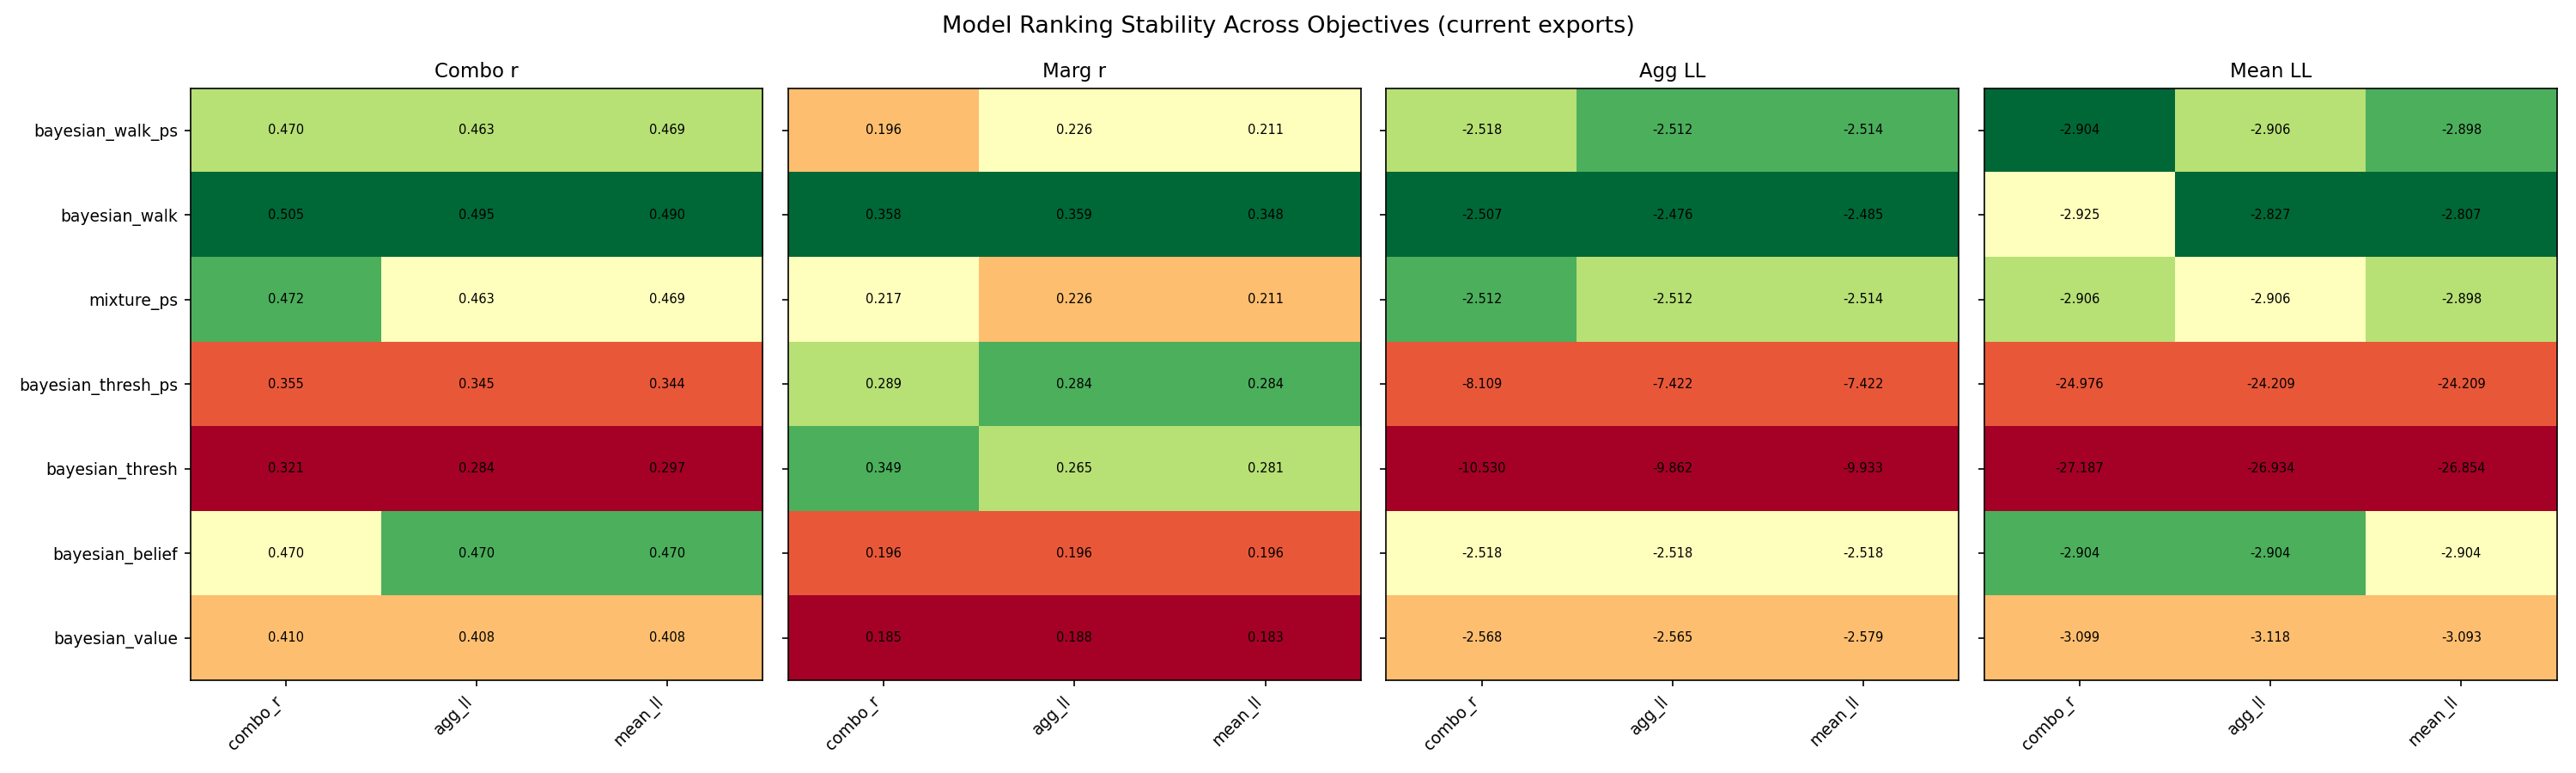
\includegraphics[width=\linewidth]{fig_model_ranking.png}
\caption{Model comparison heatmap: rows are the seven models, columns
are the four evaluation metrics, and cells show the metric value when the
model was fit under each of three different objectives (Pearson
combo-$r$, aggregate log-likelihood, and mean log-likelihood). The
\textsc{bayesian\_walk} model (row 2) is the only model that beats the
parameter-free \textsc{bayesian\_belief} baseline on every metric. The
threshold variants suffer catastrophic log-likelihood because the
threshold gate zeros out switches that humans nonetheless make. PS
(posterior-sampling) variants converge to the belief baseline because
they ignore the value function.}
\label{fig:ranking}
\end{figure*}

Three additional patterns emerge from this comparison.

\emph{Posterior-sampling variants collapse to the belief baseline.} The
walk-PS, threshold-PS, and mixture-PS models all settle into solutions
that are essentially identical to the parameter-free Bayesian-Belief
model (combo-$r$ within $0.003$). Without access to a value function,
these models cannot distinguish "I should switch towards a higher-value
role" from "the marginal posterior still favours my current role." This
provides quantitative evidence that humans \emph{do} consult the
expected-value structure of the game, not merely the posterior over
teammates.

\emph{Pure value-softmax over-predicts switching.} The
Bayesian-Value model fits a relatively high softmax temperature
($\tau_v \approx 13$) and still underperforms Bayesian-Belief on
combo-$r$ (0.41 vs.\ 0.47). The reason is that even a tempered
softmax over expected values predicts that humans will switch whenever
a competing role becomes value-superior. Empirically, humans
do not---hence the need for an explicit stickiness term.

\emph{Hard thresholds are the wrong inductive bias.} Both threshold
models suffer catastrophic log-likelihood (mean-LL $\approx -25$),
because the threshold gate concentrates mass on the previous role
whenever no competing role exceeds the value threshold by $\delta$. Any
observed switch that the model considers ``not worth it'' is then
assigned probability zero (up to a numerical floor). This penalises the
sizeable fraction of human switches that are not justified by a large
expected-value gap.

\subsection*{Bayesian-Walk tracks the human role distribution across
environments.} To verify that the aggregate fit is not an artefact of
averaging over heterogeneous environments, we computed the per-stage
human role distribution separately for the five environment
configurations with the largest sample sizes ($n=14$--$15$ teams each)
and compared it against the Bayesian-Walk and Bayesian-Belief
predictions (Fig.~\ref{fig:qualitative}). The Walk model reproduces both
the qualitative shape of the human distribution (e.g.\ Fighter-heavy
when stats favour Fighters; Medic-heavy when stats favour Medics) and
the gradual stage-to-stage drift seen in the human data, whereas the
belief-only model produces flatter, less stage-sensitive distributions.

\begin{figure*}[t!]
\centering

\includegraphics[width=\linewidth]{fig_qualitative_by_env.png}
\caption{Aggregate role-choice distribution (Fighter / Tank / Medic) at
each stage in the five most-sampled environments. Top row: humans;
middle row: Bayesian-Walk predictions; bottom row: Bayesian-Belief
predictions. The stat profile under each environment label denotes the
three players' (STR/DEF/SUP) tuples; the three-letter code names the
stat-optimal role assignment. The Walk model tracks both the
position of the modal role and its gradual drift across stages; the
belief-only model produces broader, less stage-sensitive distributions.}
\label{fig:qualitative}
\end{figure*}

\subsection*{Bot rounds: humans deviate slowly and incompletely.} Bot
rounds test whether humans can override a strong prior cue (their own
stat profile) when the team-optimal assignment requires it. The two AI
bots are set to play the deviate-optimal roles, so the human must take
the remaining role---one their stats do \emph{not} favour. Across the
five treatment batches, only 52\% of humans \emph{ever} took the
deviate-optimal role within a round, and only 32\% reached it by the
final stage (Fig.~\ref{fig:bot_role}). The deviate-optimal rate did
climb stage-by-stage (23\%, 20\%, 24\%, 30\%, 37\%), with a matching
decline in stat-optimal play, but the trajectory is shallow given that
the team's interests strongly favour deviation. Bot-round win rates
correspondingly collapsed to 34\% (vs.\ 86\% for human rounds), confirming
that the deviation challenge is genuinely demanding.

\begin{figure*}[t!]
\centering

\includegraphics[width=\linewidth]{fig_bot_role_choice.png}
\caption{Per-stage breakdown of the human's role choice in bot rounds.
The dashed green line is the fraction of humans whose role matches the
deviate-optimal slot; the orange line is the fraction still playing the
stat-suggested role. Deviation increases monotonically with stage but
remains below 40\% even at stage 5, despite bot teammates playing fixed
deviate-optimal roles that should make the correct slot identifiable.}
\label{fig:bot_role}
\end{figure*}

\begin{figure}[t!]
\centering

\includegraphics[width=\linewidth]{fig_inference_accuracy.png}
\caption{Inference accuracy by stage for human rounds (left) and bot
rounds (right). Chance accuracy is 33\%. Humans infer teammates' roles
well above chance (55--70\%) across stages, with slight decay after
stage 2 in human rounds, and a noisier trajectory in bot rounds.
The high inference accuracy juxtaposed with low deviation in bot rounds
(Fig.~\ref{fig:bot_role}) suggests that the obstacle to deviation is
not the inference itself but the willingness to abandon a strong prior.}
\label{fig:inference}
\end{figure}

Inference accuracy in bot rounds was nonetheless high (62\%, 48\%, 63\%,
59\% at stages 2--5; Fig.~\ref{fig:inference}, right): humans correctly
inferred the bots' roles most of the time. The bottleneck to deviation
is therefore not perceptual or computational---the human knows what the
bots are doing---but motivational or computational-resource-related: even
with the right information, humans resist abandoning a stat-suggested
role. This is the same pattern as the in-human-round stickiness, and is
captured by the Bayesian-Walk model's $\varepsilon_s$ parameter.

\section*{Discussion}\label{sec:discussion}

We introduced an experimental paradigm for ad-hoc role specialization and
showed that human role choice in this paradigm is well-described by a
Bayesian theory-of-mind model augmented with a stickiness bias. Three
findings stand out.

\emph{Bayesian inference about teammates' roles is largely correct.}
Single-stage inference accuracy is 60--70\% across stages in both human
and bot rounds (chance = 33\%), and a Bayesian inference engine with
held-out-fitted action noise and a soft drift-to-prior memory predicts
those reports with 92\% argmax accuracy. Whatever else humans are doing,
they are running an approximately correct generative model of their
teammates' role-driven behaviour.

\emph{Role selection is sticky and value-aware.} Among the role-selection
rules we compared, the only one that reliably beats the
posterior-marginal baseline across every metric is the Bayesian-Walk
rule: an $\varepsilon$-mixture between the previously played role and a
softmax over expected utilities given the posterior. Pure
value-softmax over-predicts switching; pure posterior-marginal is
indifferent to the value structure; hard thresholds zero out switches
humans actually take. The empirical switch rate of 35--45\% and the
fitted $\varepsilon_s \approx 0.55$ are tightly aligned.

\emph{Deviation from a stat-suggested role is harder than the inference
it requires.} In bot rounds, humans accurately inferred their bot
teammates' roles, but only a third of them successfully deviated by the
final stage. The bottleneck is therefore action, not inference: humans
hold a strong prior about which role suits their stats and resist
abandoning it even when the joint optimum requires it. This is
consistent with broader findings that human decision-making favours
status-quo and habitual responses when the cost of computing an
alternative is non-trivial \cite{lieder2020resource, simon1956rational},
and connects naturally to the literature on resource-rational
contractualism \cite{trujillo2025resource, kwon2023universalization} in
which heuristics are deployed selectively rather than uniformly.

These findings extend the empirical reach of Bayesian theory-of-mind in
three directions. First, they show that the Bayesian approach scales from
two-agent settings \cite{baker2017rational, tan2019norms} to multi-agent
cooperation tasks with structured asymmetries between participants.
Second, they make precise the contribution of \emph{roles} as a level of
abstraction \cite{bakerRolesGuideRapida, bakerPeopleUseMixed2025,
mieczkowski2024specialization}: roles are not merely category labels but
\emph{decision variables}, the things over which agents form posteriors
and the things they choose. Third, they identify a specific quantitative
form of bounded rationality---behavioural stickiness with $\varepsilon_s
\approx 0.55$---that captures the systematic departure of human role
choice from idealised Bayesian optimality.

\emph{Limitations and future work.} (i) Our task has only three roles
and three players; whether the Bayesian-Walk decision rule scales to
larger role spaces (with the corresponding combinatorial explosion in
the joint posterior) is an open question. (ii) We aggregate over
individuals when reporting model fits; preliminary individual-level
fits suggest substantial heterogeneity, with some participants better
explained by a pure walk model and others by the value-aware Walk,
mirroring findings of mixed-strategy use in role inference
\cite{bakerPeopleUseMixed2025}. A planned follow-up will report
participant-level model assignments and their relationship to
demographic and task-performance covariates. (iii) Our environment uses
only deterministic role-conditional action policies; richer policies
(e.g.\ probabilistic mixing within a role) would test whether humans
maintain a posterior over policy parameters as well as role identity.
(iv) Finally, the bot-round deviation task could be parametrised to
quantify exactly how strong a value gradient is required to overcome a
given amount of stat-prior support, yielding a psychometric function for
ad-hoc role flexibility.

Taken together, our results provide a quantitative foundation for the
study of ad-hoc role specialization as a tractable cognitive
problem. People do not appear to coordinate by sharing a plan; they
appear to run a Bayesian model of who their teammates are, and they
move---sluggishly but reliably---toward the role that makes the team
work.

\matmethods{
\subsection*{Participants.} We recruited 150 adults from the Prolific
crowdsourcing platform \cite{nasprolific}, restricted to participants
$\geq 21$ years of age and fluent in English. Each participant
completed a self-paced tutorial, a comprehension check (repeated until
passed), and a sequence of cooperative game rounds. Compensation was
paid at a fixed hourly rate plus a small completion bonus, irrespective
of outcome. Procedures were approved by the relevant institutional
review board.

\subsection*{Experimental platform.} The task was implemented in the
Empirica framework \cite{empirica2021}, which supports synchronous
multi-player browser-based experiments with built-in dropout handling
and per-round timing. The codebase, environment configurations, and raw
data exports are publicly available (see Data Availability). Three
players were grouped into a game by Empirica's matching logic; if a
player dropped out (failed a stage timer or closed the browser), their
role was auto-assigned by a fallback rule, and the entire game was
flagged for exclusion from human-round analyses.

\subsection*{Stat profiles and round configuration.} A stat profile
$\theta_i = (\mathrm{STR}_i, \mathrm{DEF}_i, \mathrm{SUP}_i)$ assigns
integer multipliers to the Fighter, Tank, and Medic actions
respectively. We used a base set of profiles
$\{(4,1,1), (1,4,1), (1,1,4), (2,2,2)\}$ to span asymmetric and
symmetric configurations. Each round drew a triple of stat profiles and
an optimal-role-assignment label from a precomputed configuration list,
together with the boss's attack-intent sequence (which is common
knowledge). Bot rounds additionally specified the two bots' fixed
roles, which were always set to the deviate-optimal slots.

\subsection*{Game dynamics.} On each turn, the boss either attacks (1)
or pauses (0) according to the publicly disclosed intent sequence. The
three players' actions resolve simultaneously: attack damages are
summed into the boss; the maximum defender's DEF reduces incoming
damage if the boss attacks; total SUP heals the team back toward
$\mathrm{TeamMaxHP}$. The boss has a fixed HP pool and a fixed
per-attack damage; both team and boss HP are capped at their respective
maxima. A round ends in WIN if boss HP $\leq 0$, LOSE if team HP $\leq 0$,
or TIMEOUT after the fifth stage. Each stage is two turns; players
choose a role at the start of every stage and may not change it
mid-stage.

\subsection*{Value matrices.} For every stat-profile/role-combination
configuration used in the experiment, we precomputed the team value
function $V(r_1,r_2,r_3, \text{intent}, \text{thp}, \text{ehp})$ by
value iteration on the underlying tabular MDP. These are the values
used by the Bayesian-Value, Bayesian-Walk, and Bayesian-Threshold
models. Value matrices are stored in
\texttt{analysis/data/human\_envs\_value\_matrices/} and are loaded
deterministically by the model-fitting pipeline; a missing matrix raises
an error rather than silently dropping the affected records.

\subsection*{Data filtering.} Out of 50 games (1200 player-rounds), 16
games (32\%) contained at least one dropout participant. Those games
are excluded entirely from the analyses reported in the main text.
Within the remaining 34 games, we retained team-rounds in which all
three players were present and no stage was auto-submitted by the
dropout fallback. This yielded 187 clean human team-rounds and 258
clean human bot-rounds.

\subsection*{Inference fitting (Stage 1).} The Bayesian inference
engine has three free parameters: the prior temperature $\tau_p$, the
action noise $\varepsilon$, and the cross-stage memory parameter
$\beta$. We searched a coarse grid over each parameter and evaluated
the inference engine against the human inference reports (stage-by-stage
guesses of teammates' previous-stage roles). The best configuration
was $\tau_p = 4.64$, $\varepsilon = 0.062$, $\beta = 0.50$ (drift-to-prior).
This single set of inference parameters is used by all Stage-2 models.

\subsection*{Role-selection fitting (Stage 2).} For each of the seven
models in Table~\ref{tab:models}, we fit its remaining parameters by
maximising the Pearson correlation between the model's predicted joint
role-combination distribution and the empirical distribution over the
204 fitting team-rounds. We additionally evaluated each fit under
aggregate log-likelihood and mean log-likelihood objectives; the
ranking is stable across all three (Fig.~\ref{fig:ranking}). The 17
unique stat-profile/role-combination configurations in the data each
require a precomputed value matrix; configurations missing a matrix
were dropped before fitting (no drops were required in the final
analysis).

\subsection*{Implementation.} All analyses were implemented in Python
3.11 with NumPy 1.26 and SciPy 1.13. The full code is released alongside
the data; the key inference and model definitions live in
\texttt{analysis/shared/inference.py} and
\texttt{analysis/experiments/2026-05-12-current-export-metric-comparison/}.}

\showmatmethods{}

\dataavail{Anonymised participant data, environment configurations, and
all analysis code are available at the project repository
(\url{https://github.com/jolow99/bayesian-role-specialization}).
Stage-1-fitted inference parameters and Stage-2 model fits are
deterministically reproducible from the released code.}

\acknow{We thank the participants who took part in the study. We thank
members of the National University of Singapore CISL group for helpful
discussions during the development of this work.}

\showacknow{}


\bibsplit[3]

% Bibliography
\bibliography{references}

\end{document}
